\documentclass[a4paper, 12pt]{article}

\usepackage[top=2cm, bottom=2cm, left=2.5cm, right=2.5cm]{geometry}
\usepackage[utf8]{inputenc}
\usepackage{array}
\usepackage{cancel}
\usepackage{graphicx}
\usepackage{amsmath}

\graphicspath{{img/}}

\begin{document}
\begin{flushleft}
\includegraphics{logo}\\
\textbf{UNIVERSIDADE ESTADUAL DE PONTA GROSSA} \\
SISTEMA UNIVERSIDADE ABERTA DO BRASIL - UAB \\
\underline{Licenciatura em Matemática | Polo UAB em Jacarezinho}\end{flushleft} 
\textbf{ALUNO:} Ricardo Medeiros da Costa Junior   \textbf{RA:} 151774301 \\
\textbf{DISCIPLINA:} Fundamentos da Matemática III \\
\textbf{ATIVIDADE:} Atividade 8 - Tarefa: Equações Polinomiais\\
\textbf{TUTOR(A)}: Julio Cezar de Souza\\
\textbf{PERÍODO:} Terceiro\\
\begin{enumerate}
\item Elabore cinco questões envolvendo a obtenção das raízes de equações polinomiais.\\
  \begin{enumerate}
  \item Determine as raízes da equação $x^{3}+x^2-4x+6=0$, sabendo que $1+i$ é uma de suas raízes. \\\\
    \centering
    \begin{tabular}{c c c c c}
    1+i & \textbar 1 & 1 & -4 & 6 \\
    1-i & 1 & 2+i & -3+3i & 0 \\
    &  1 & 3 & 0
    \end{tabular}
    $$ x + 3 = 0 \Rightarrow $$
    $$ x = -3 $$
    $$ \boxed{S=\{-3, 1-i, 1+i\}}$$

  \item Determine as raízes inteiras da equação $3x^3-2x^2-7x-2=0$ \\\\
    Divisores de 2: -1, 1, -2, 2\\\\
    $$3(1)^3-2(1)^2-7(1)-2=0 \Rightarrow $$
    $$3-2-7-2=0 \Rightarrow $$
    $$3-11 \ne 0$$\\\\
    
    $$3(-1)^3-2(-1)^2-7(-1)-2=0 \Rightarrow $$
    $$-3-2+7-2=0 $$\\\\

    $$3(2)^3-2(2)^2-7(2)-2=0 \Rightarrow $$
    $$3(8)-2\cdot4-14-2=0 \Rightarrow $$
    $$24-8-14-2 = 0$$\\\\

    $$3(-2)^3-2(-2)^2-7(-2)-2=0 \Rightarrow $$
    $$3(-8)-2\cdot4+14-2=0 \Rightarrow $$
    $$-24-8+12 \ne 0$$

    Raízes inteiras: $$ \boxed{\{-1,2\}}$$
  \item Sabendo que 5 é raiz da equação  $x^3-5x^2+x +k = 0$, pede-se:
    \centering
    \begin{tabular}{t t}
    a) O valor de k & b) Resolver a equação
    \end{tabular}
    \begin{description}
    \item[a) Valor de k:]\\\\
      $$(5)^3-5(5)^2+5+k=0 \Rightarrow $$
      $$ \cancel{125}-\cancel{125}+5+k=0 \Rightarrow $$
      $$ \boxed{k = -5}$$\\\\
    \item[b) Resolver a equação]\\\\
    \centering
    \begin{tabular}{c c c c c}
    5 & \textbar 1 & -5 & 1 & -5 \\
      & 1 & 0 & 1 & 0 \\    
    \end{tabular}\\\\
    $$x^2+1=0 \Rightarrow $$
    $$x^2=-1$$
    $$x= \pm \sqrt{-1} \Rightarrow$$
    $$x= \pm \sqrt{1(-1)} \Rightarrow$$
    $$x= \pm \sqrt{1}\cdot\sqrt{i^2} \Rightarrow$$
    $$x= \pm \sqrt{1}\cdot i \Rightarrow$$
    $$x= \pm i $$
    $$\boxed{S=\{-i, i, 5\}}$$
    \end{description}
  \item Resolva a equação $x^3+x^2-5x-5=0$
    $$(-1)^3+(-1)^2-5(-1)-5=0 \Rightarrow$$
    $$-1+1+5-5=0$$ 
    \centering
    \begin{tabular}{c c c c c}
    -1 & \textbar 1 & 1 & -5 & -5 \\
      & 1 & 0 & -5 & 0 \\    
    \end{tabular}\\\\
    $$x^2-5=0$$
    $$x^2=5$$
    $$x= \pm \sqrt{5}$$\\\\
    $$\boxed{S=\{-\sqrt{5},-1,\sqrt{5}\}}$$
  \item Resolva a equação $x^4-7x^3+9x^2+7x-10=0$
    $$(1)^4-7(1)^3+9(1)^2+7(1)-10=0 \Rightarrow$$
    $$1-7+9+7-10=0$$
    \centering
    \begin{tabular}{c c c c c c}
    1 & \textbar 1 & -7 & 9 & -10 \\
      & 1 & -6 & 3 & 10 & 0 \\    
    \end{tabular}\\\\
    $$x^3-6x^2+3x+10=0 \Rightarrow $$
    $$(-1)^3-6(-1)^2+3(-1)+10=0 \Rightarrow $$
    $$-1-6-3+10=0$$
    \centering
    \begin{tabular}{c c c c c}
    -1 & \textbar 1 & -6 & 3 & 10 \\
      & 1 & -7 & 10 & 0 \\    
    \end{tabular}\\\\
    $$x^2-7x+10=0$$
    $$S=7=2+5$$
    $$P=10=2\cdot5$$
    $$\boxed{S=\{1,-1,2,5\}}$$
    
    
    
  \end{enumerate}
\item Em seguida apresente graficamente as soluções reais. \\
    \begin{figure}[h!]
    \centering
    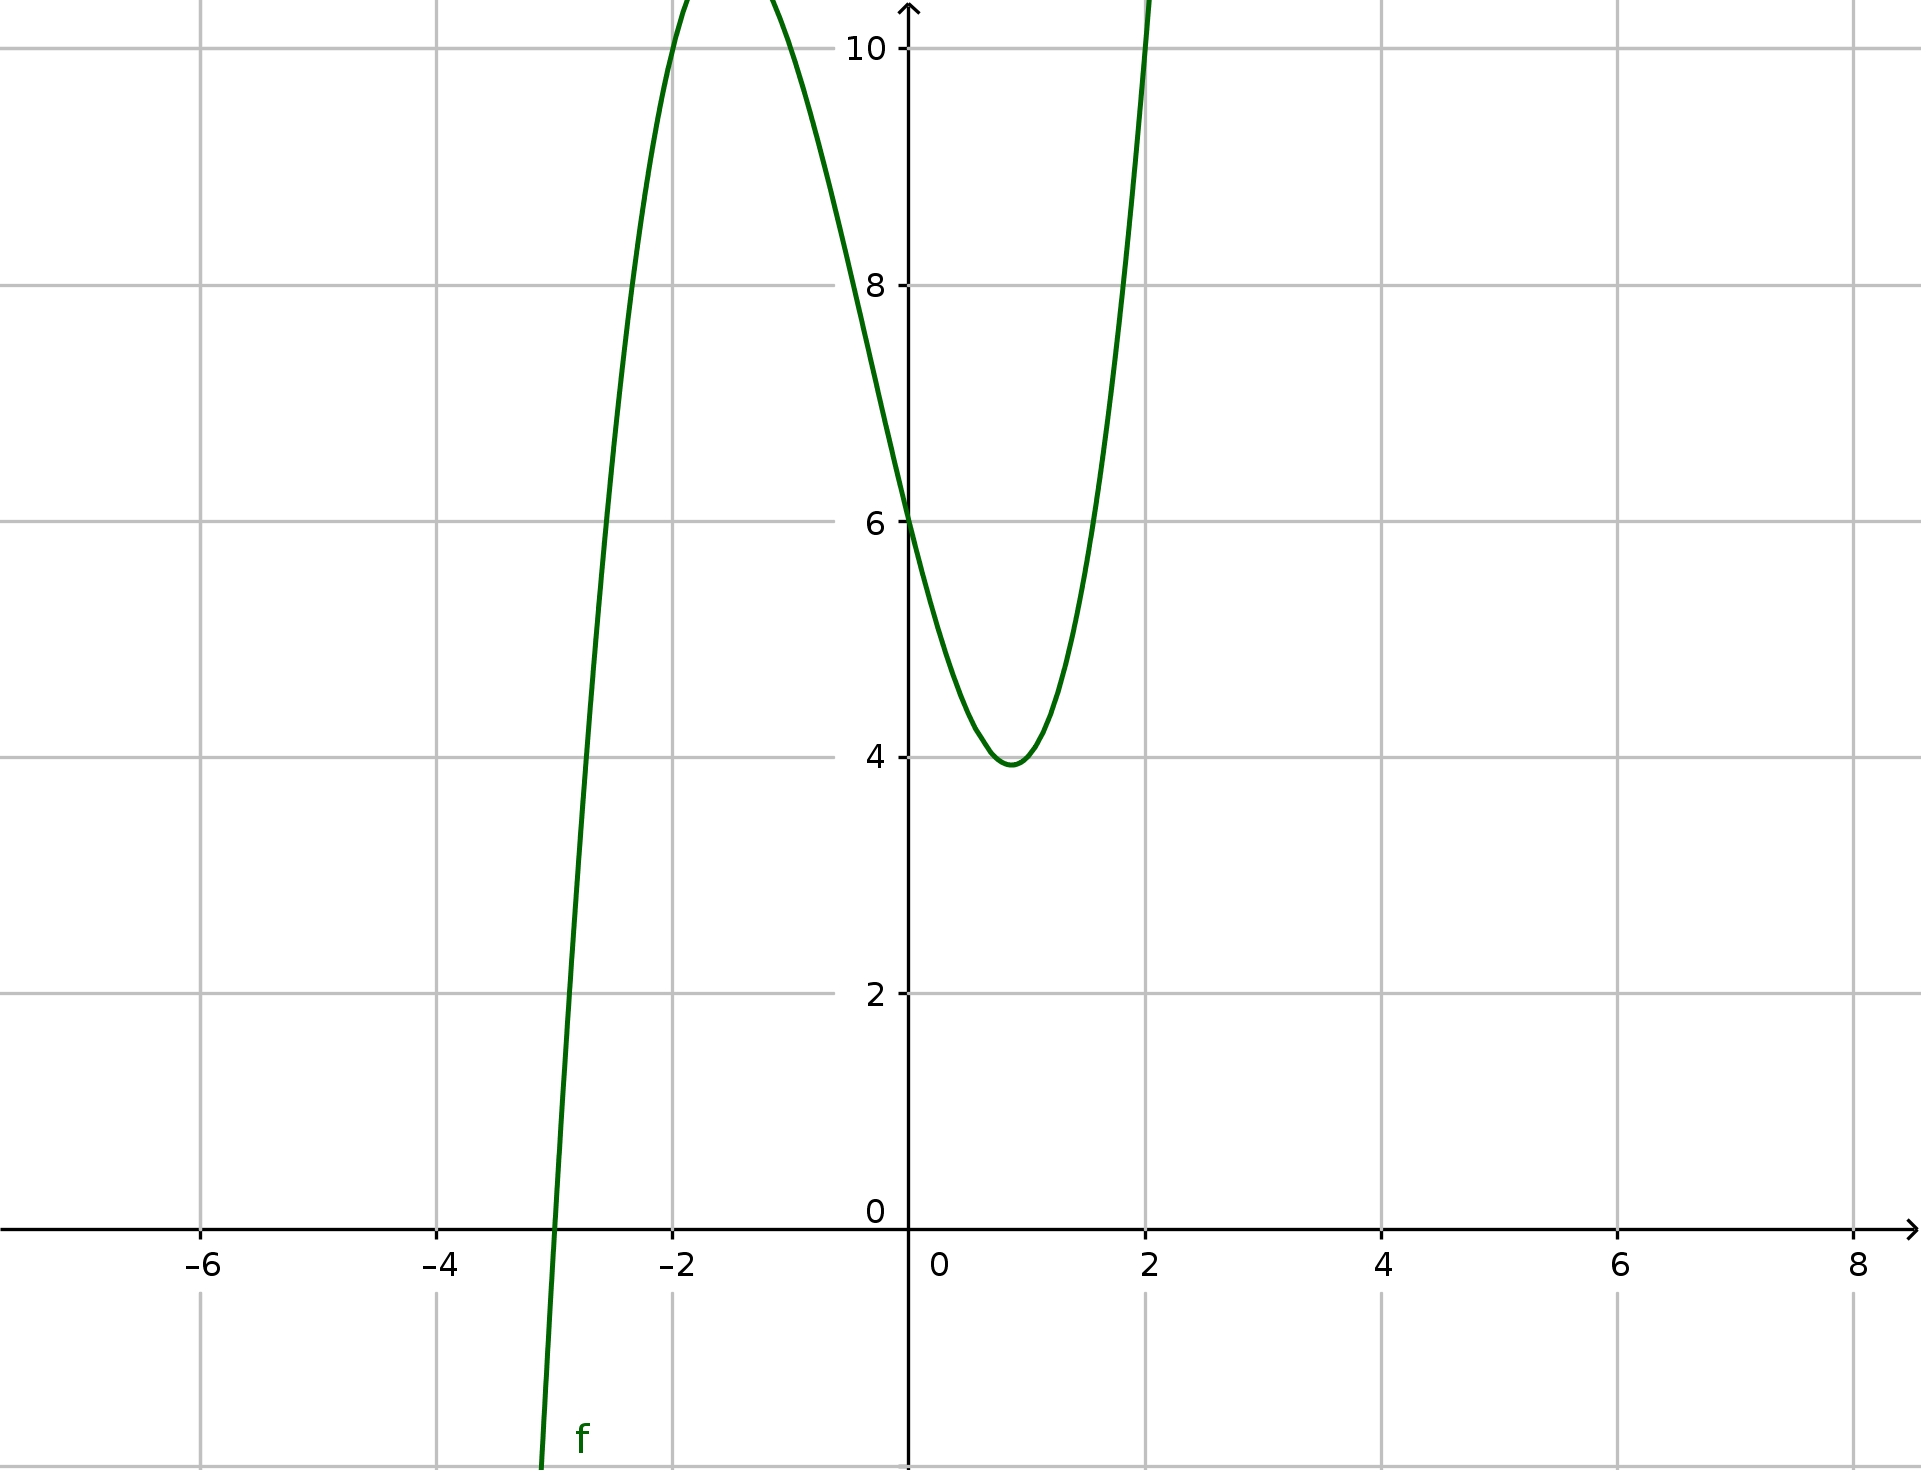
\includegraphics[width=120mm]{img1.png}
    \caption{Exercício 1}
    \end{figure}

    \begin{figure}[h!]
    \centering
    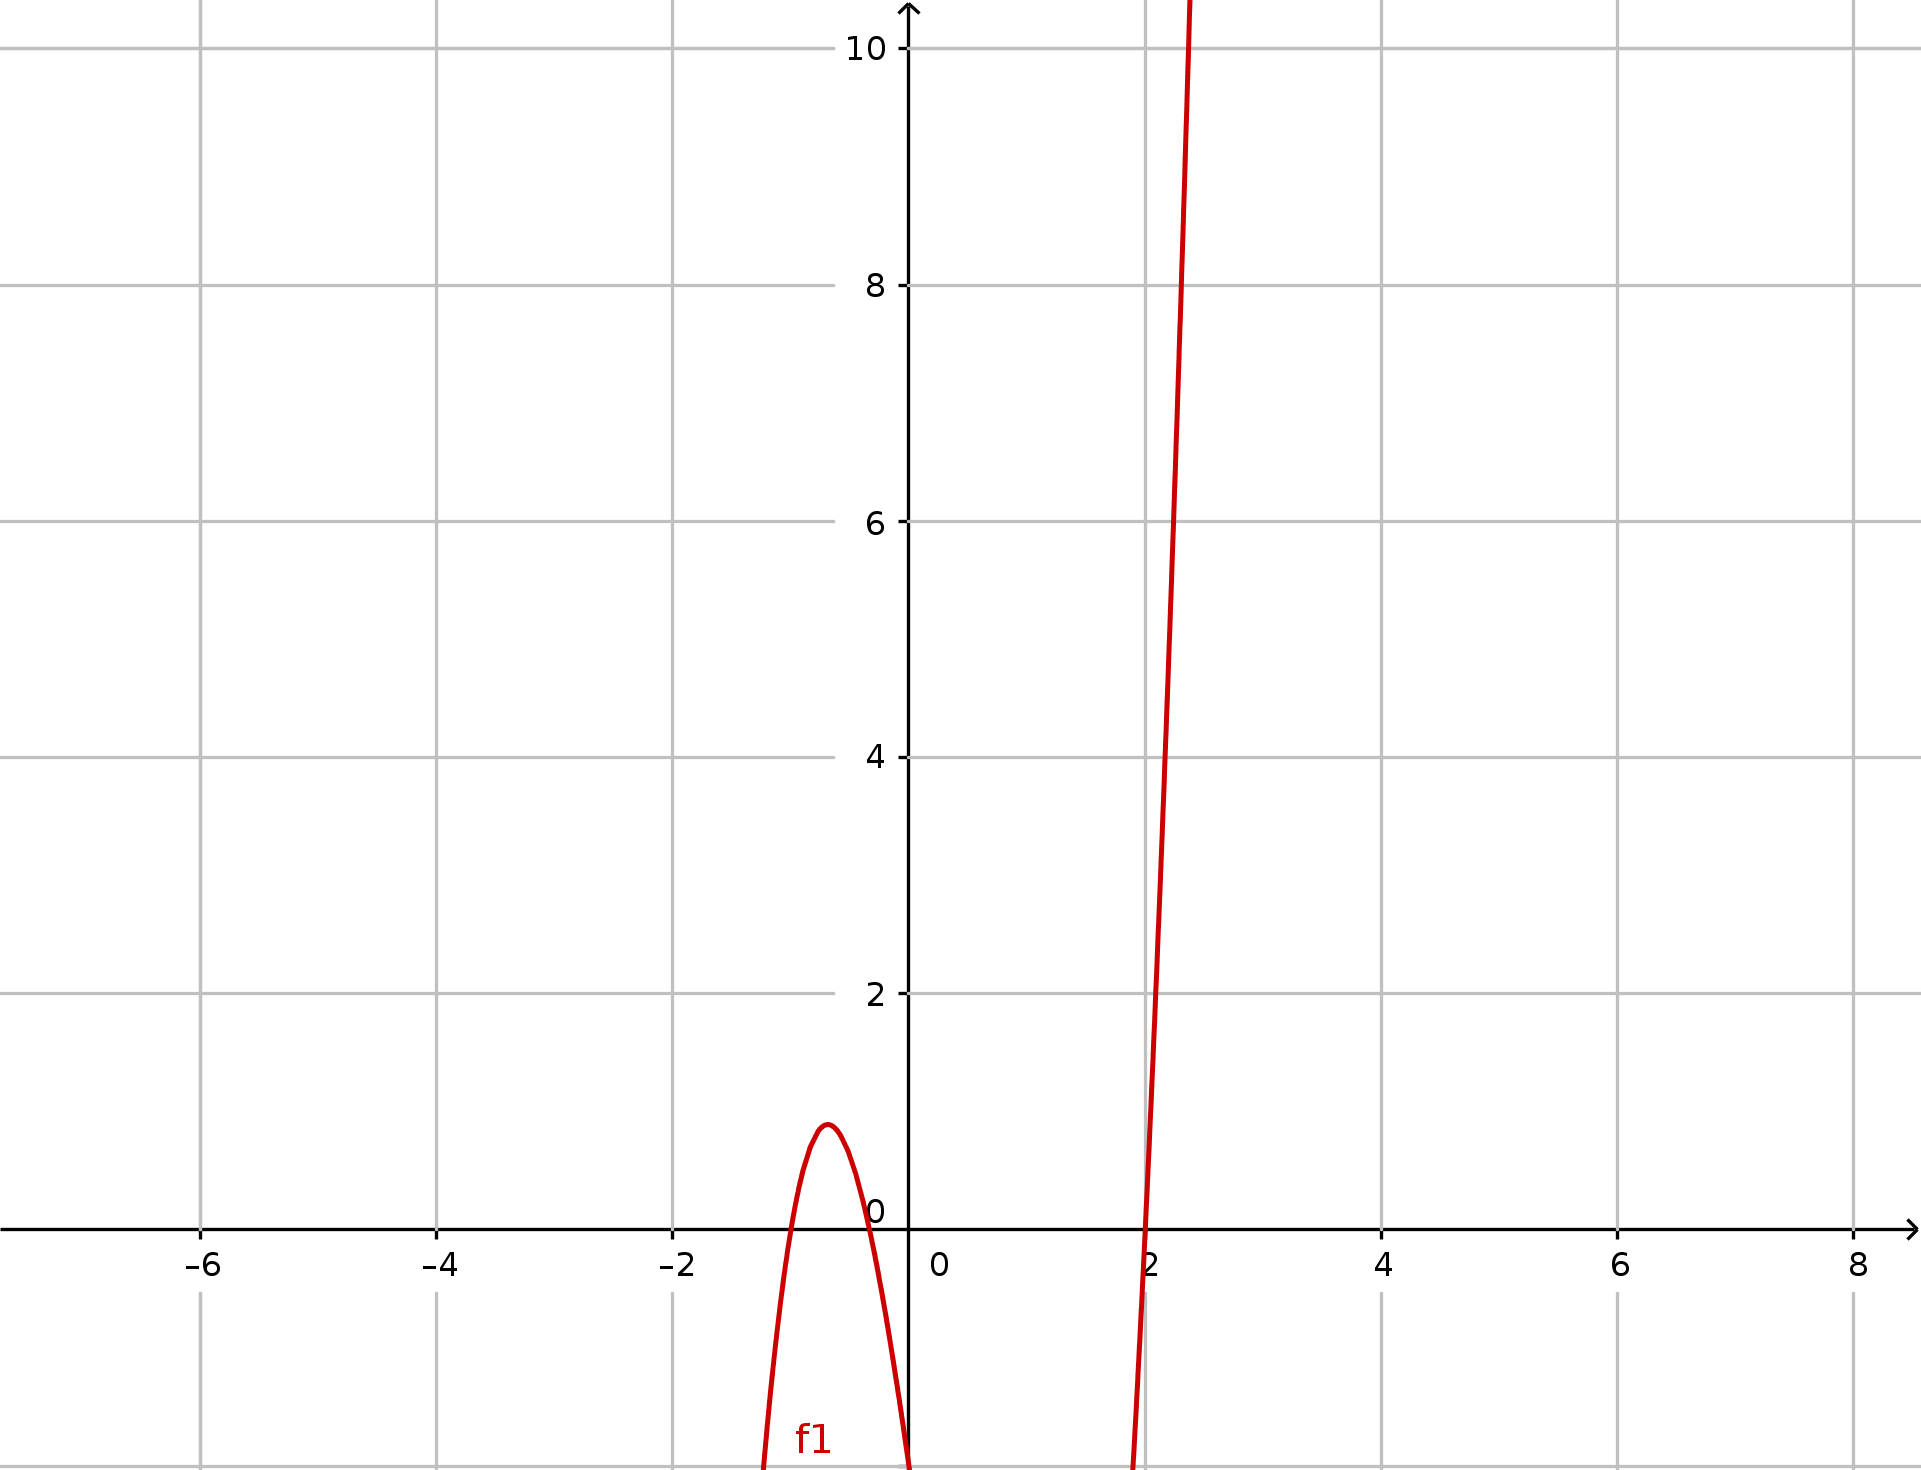
\includegraphics[width=120mm]{img2.png}
    \caption{Exercício 2}
    \end{figure}

    \begin{figure}[h!]
    \centering
    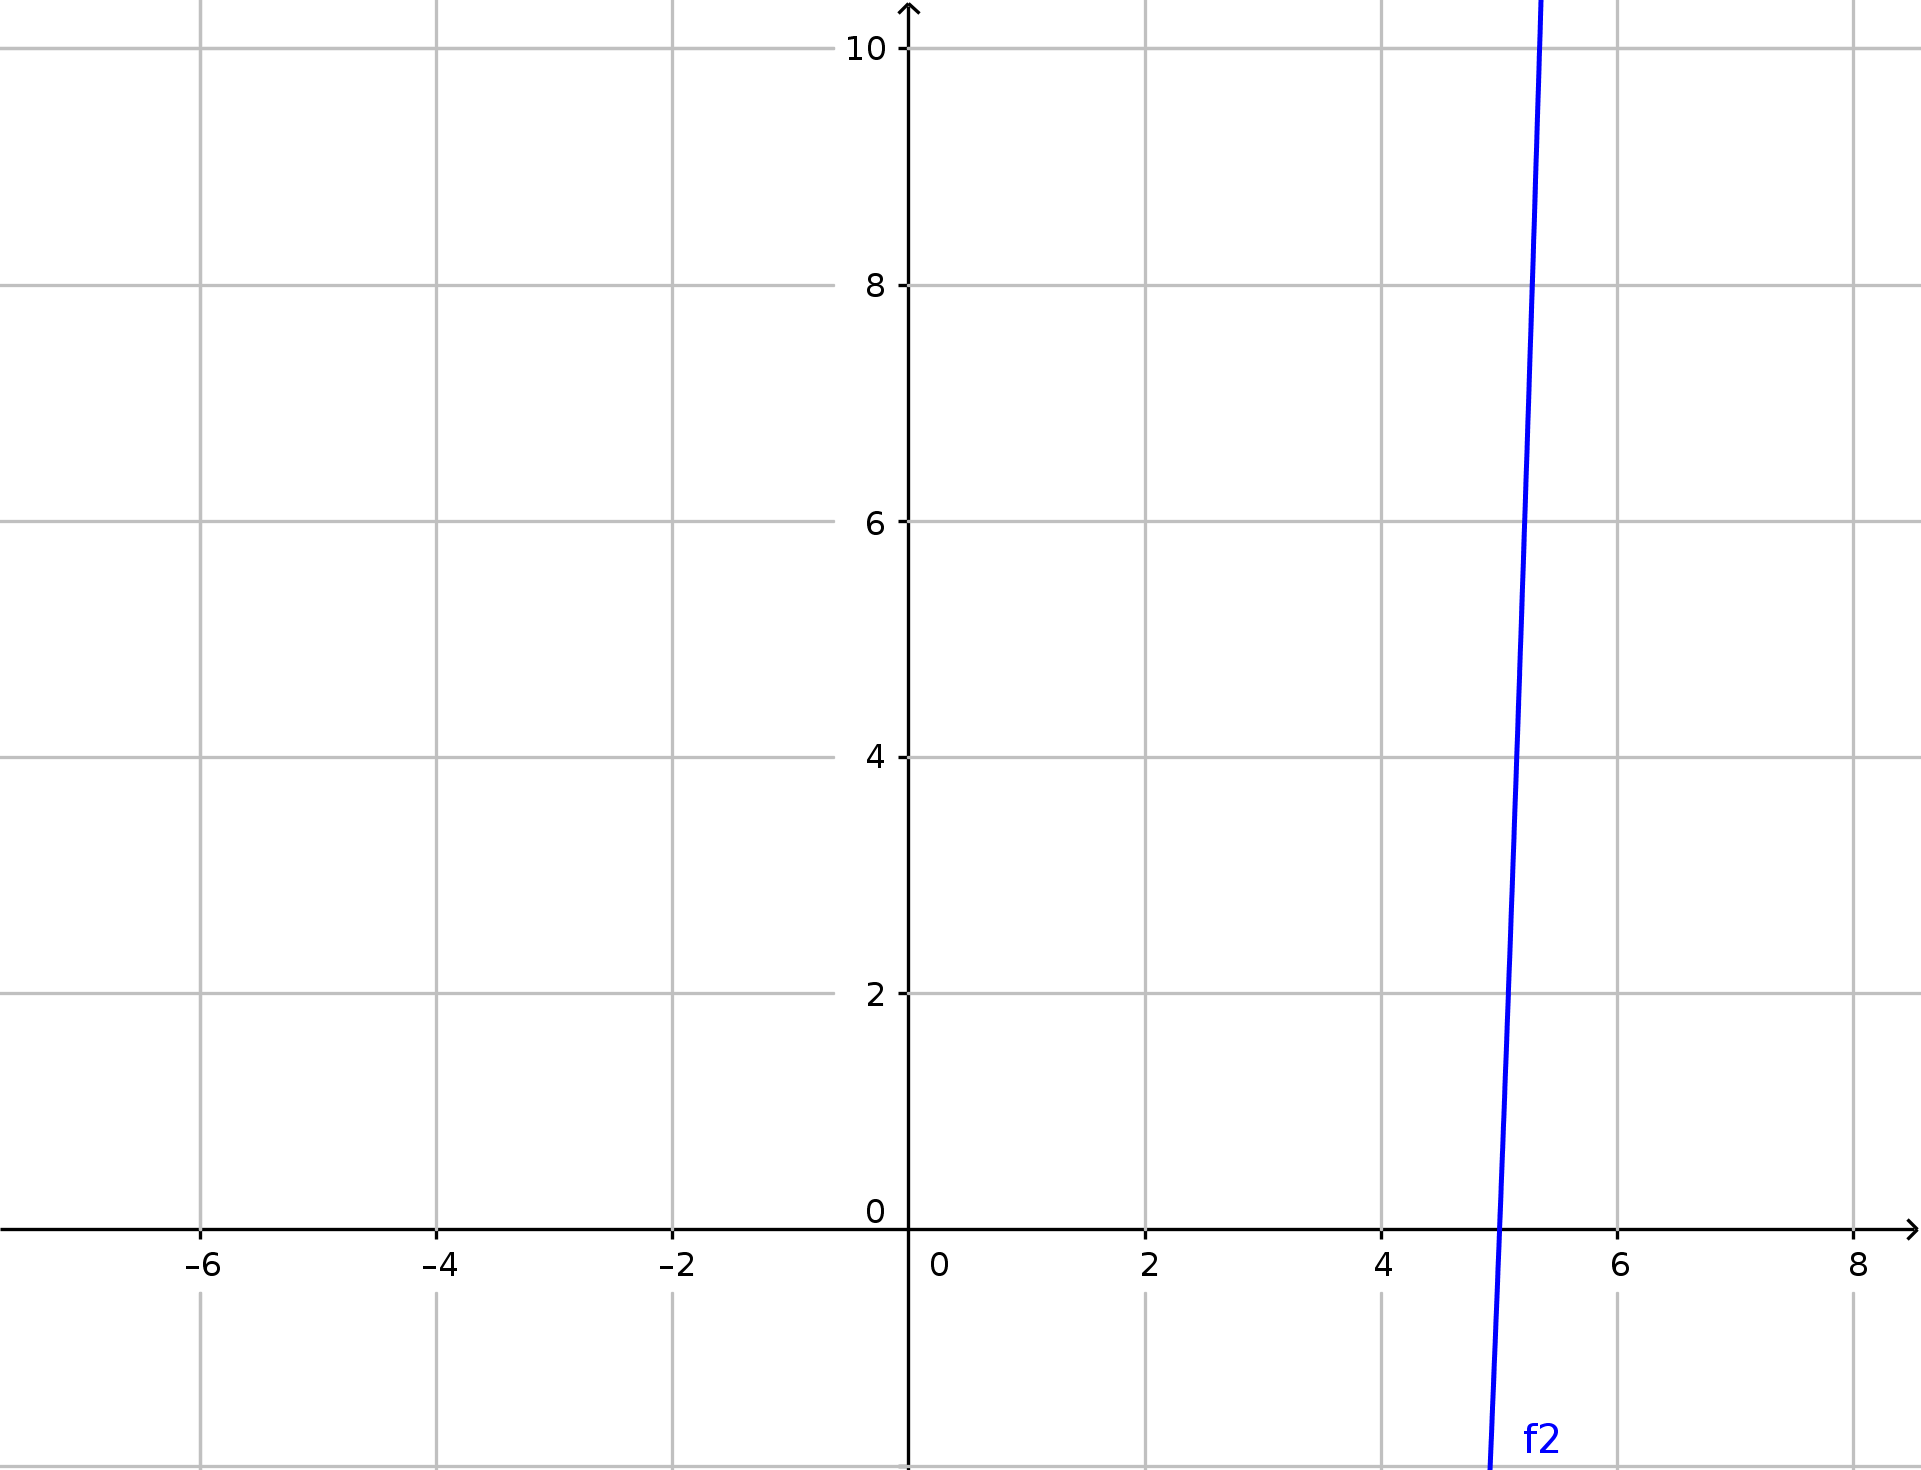
\includegraphics[width=120mm]{img3.png}
    \caption{Exercício 3}
    \end{figure}

    \begin{figure}[h!]
    \centering
    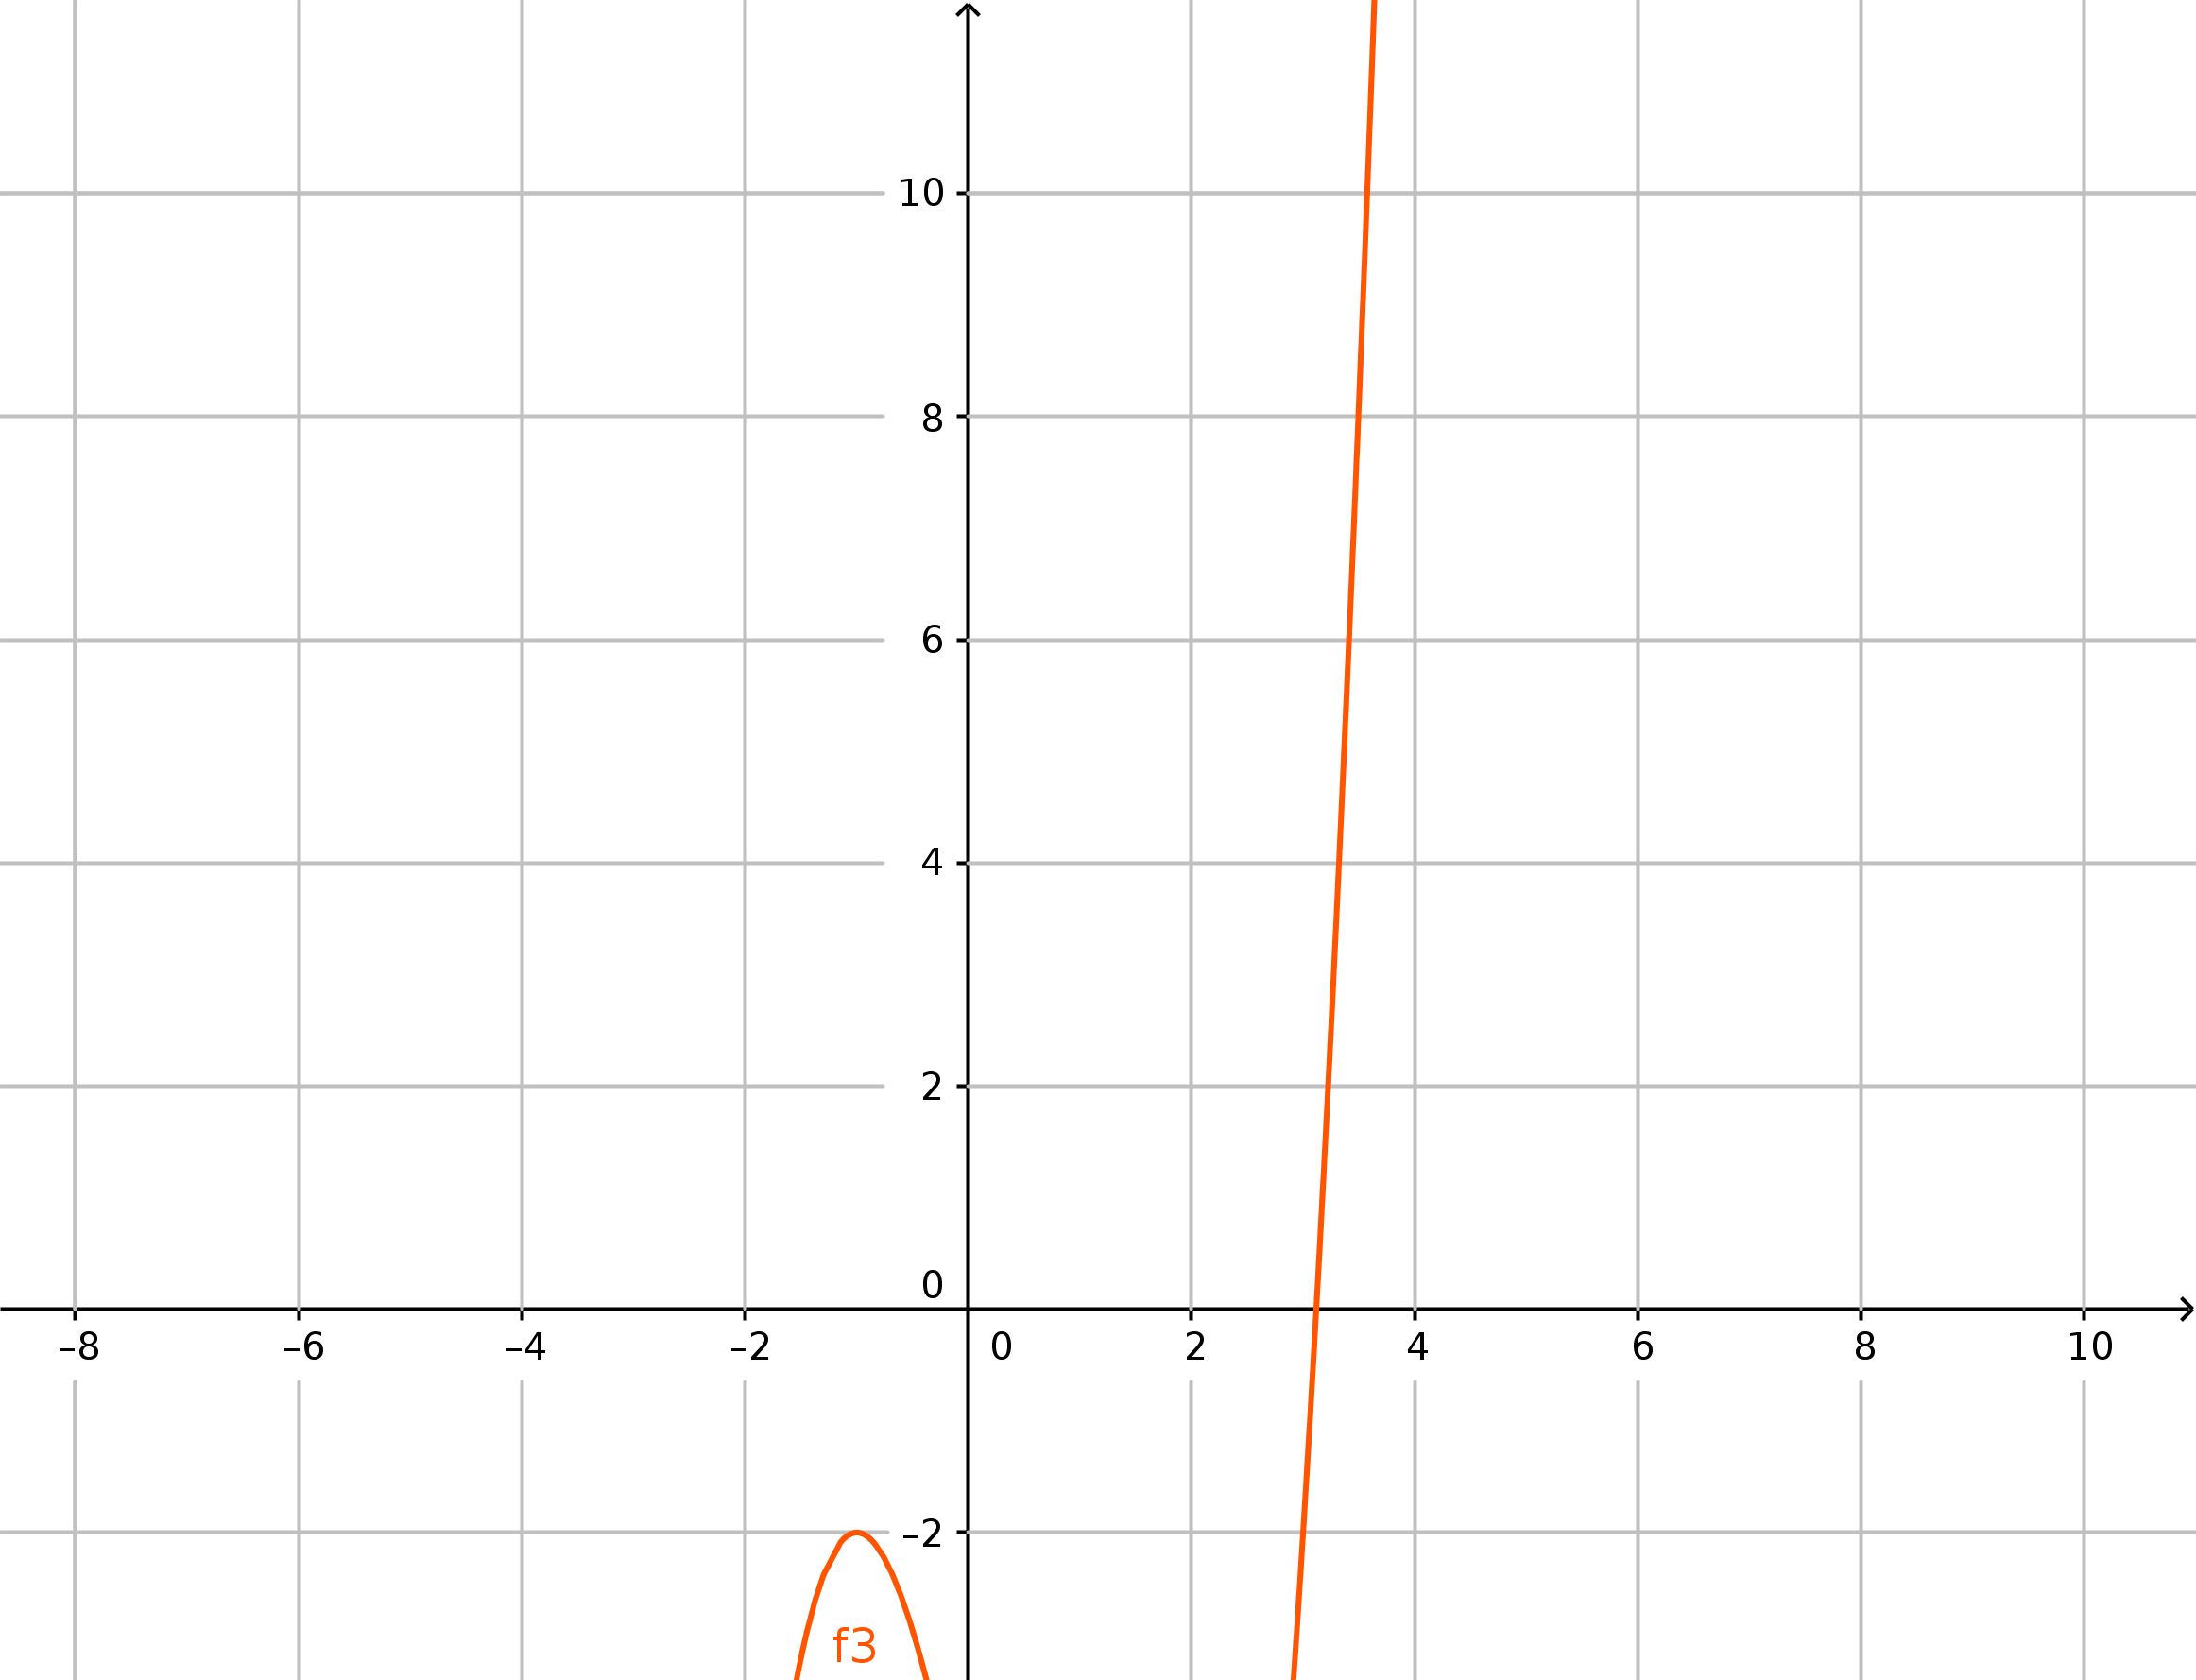
\includegraphics[width=120mm]{img4.png}
    \caption{Exercício 4}
    \end{figure}

    \begin{figure}[h!]
    \centering
    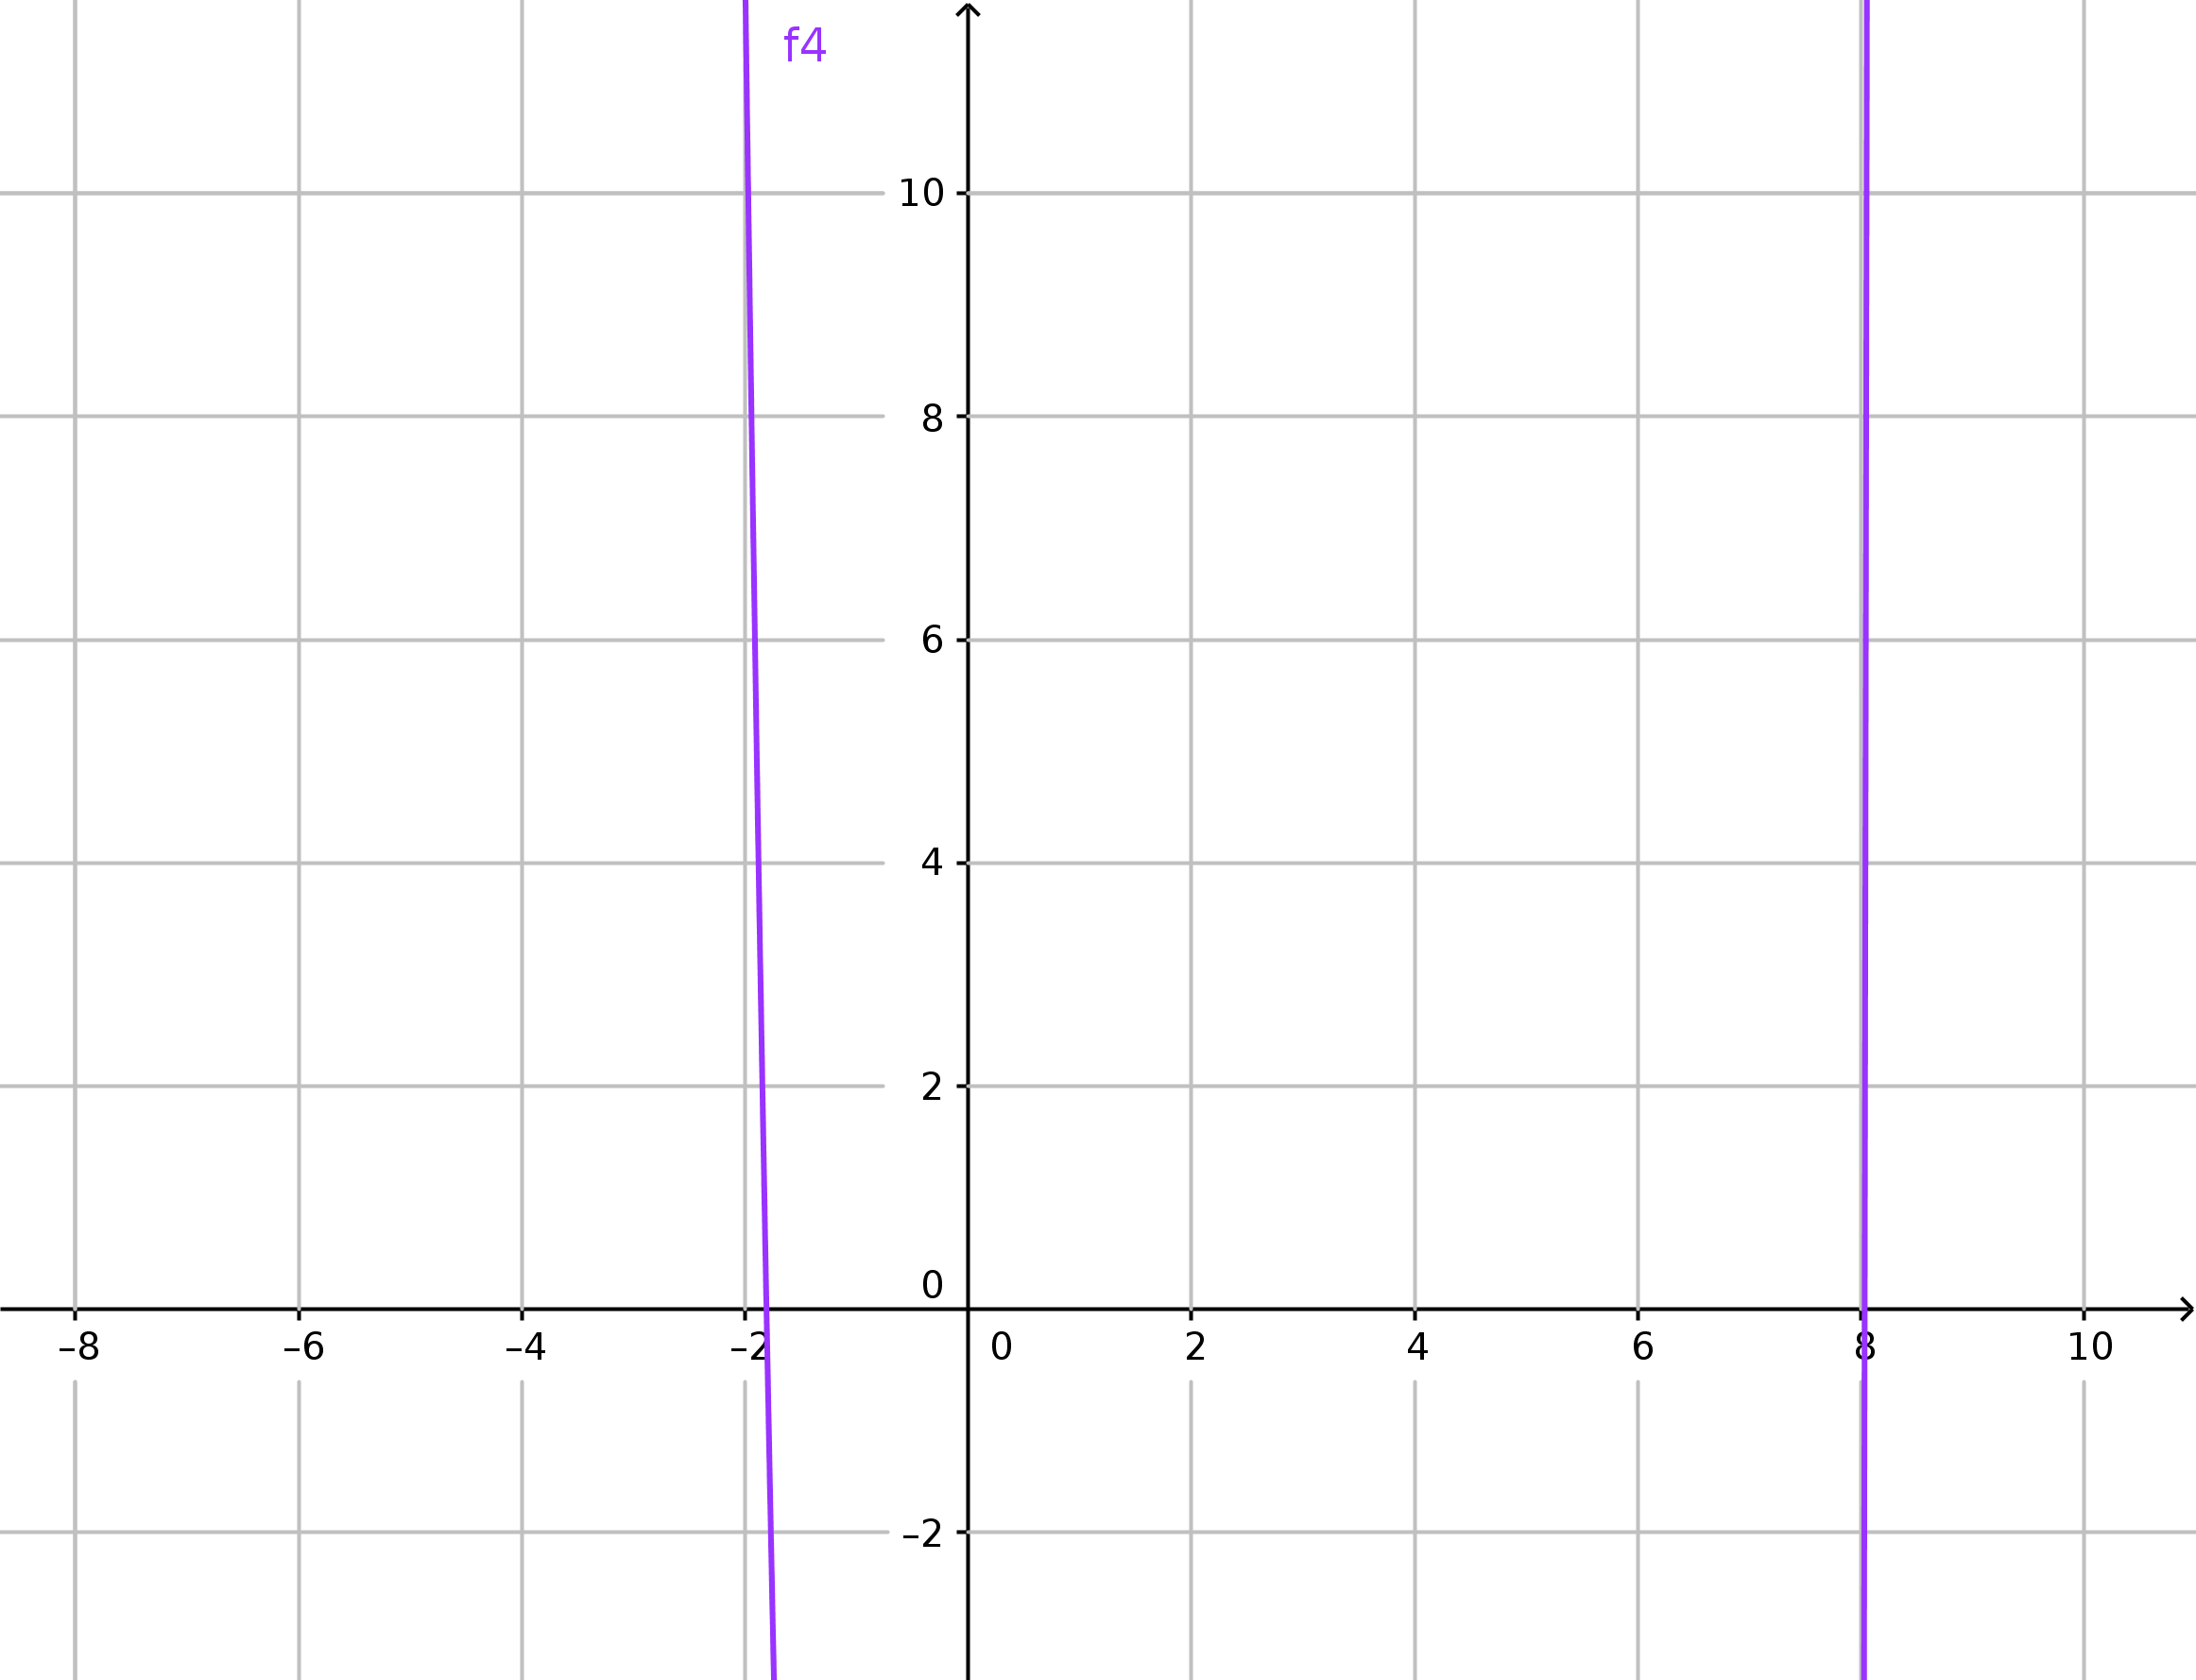
\includegraphics[width=120mm]{img5.png}
    \caption{Exercício 5}
    \end{figure}

\end{enumerate}
\end{document}
